\begin{figure}
  \centering
    \scalebox{1}
    {  \begin{sequencediagram}
    \newthread{A}{\shortstack{User \\ Browser \\ \\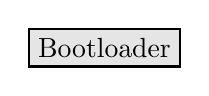
\begin{tikzpicture}
\node [fill=gray!20,draw=black,thick ,align=center] {Bootloader};
\end{tikzpicture}}}{}
    \newinst[1]{B}{\shortstack{Servidor de \\ aplicaciones \\ \\ \begin{tikzpicture}
\node [copy shadow,fill=gray!20,draw=black,thick ,align=center] {Procesos};
\end{tikzpicture}}}{}
    \newinst[1]{C}{\shortstack{Servidor de \\  de Datos \\ \\\begin{tikzpicture}[shape aspect=.5]
\tikzset{every node/.style={cylinder, shape border rotate=90, draw,fill=gray!25}}
\node  at (1.5,0) {BD};
\end{tikzpicture}}}{}    
    \begin{call}{A}{}{B}{}
    \end{call}
    \begin{call}{B}{}{C}{}
    \end{call}
  \end{sequencediagram}
  }
\caption{Loading OBJKT with bootloader} 
\end{figure}